\documentclass[a4paper, journal]{IEEEtran}
\usepackage[margin=0.75in]{geometry}
\IEEEoverridecommandlockouts
% The preceding line is only needed to identify funding in the first footnote. If that is unneeded, please comment it out.
\usepackage{cite}
\usepackage{amsmath,amssymb,amsfonts}
\usepackage{algorithmic}
\usepackage{graphicx}
\usepackage{textcomp}
\usepackage{listings}
\usepackage{xcolor}

\lstset{
  language=Python,
  breaklines=true,
  breakatwhitespace=true,
  basicstyle=\ttfamily\footnotesize,
  keywordstyle=\color{blue},
  commentstyle=\color{gray},
  stringstyle=\color{red},
  captionpos=b,
  frame=single,
  showstringspaces=false,
  tabsize=4
}


\hyphenation{op-tical net-works semi-conduc-tor IEEE-Xplore}
\def\BibTeX{{\rm B\kern-.05em{\sc i\kern-.025em b}\kern-.08em
    T\kern-.1667em\lower.7ex\hbox{E}\kern-.125emX}}
\usepackage{balance}
\begin{document}

\title{Perceptron Learning Algorithm}
\author{
\IEEEauthorblockN{Dinanath Padhya\IEEEauthorrefmark{1}, Krishna Acharya\IEEEauthorrefmark{2}} \\
\IEEEauthorblockA{\IEEEauthorrefmark{1}THA078BEI010 \quad \IEEEauthorrefmark{2}THA078BEI020\\
Department of Electronics, Communication and Information Engineering\\
Thapathali Campus, IOE, Tribhuvan University, Nepal\\
}}

\maketitle

\begin{abstract}
This report presents a comprehensive exploration of the Perceptron Learning Algorithm applied to fundamental logic functions, including AND, OR, and NOT gates, and examines its inherent limitation with the XOR operation. Beginning with a detailed theoretical background, we introduce the various activation functions and perceptron model. The Heaviside activation function, followed by the learning rule that iteratively adjusts weights and bias based on prediction errors. We also explore about sigmod activation function. W.Implemented in Python using NumPy, the algorithm was trained on truth-table datasets, achieving rapid convergence for linearly separable functions. Quantitative results are provided, including final weight vectors, biases, epoch counts, and visualized decision boundaries. In contrast, the XOR gate training process fails to converge, underscoring the necessity of non-linear architectures for non-linearly separable problems. We supplement the previous experimental findings of XOR inseparability and reference historical work by Minsky and Papert. Concluding remarks highlight the perceptron utility for simple classification tasks and its limitations, motivating the progression to multi-layer networks and non-linear activation functions for complex problem domains.

\end{abstract}

\begin{IEEEkeywords}
    Perceptron, Logic Gates, XOR Problem, Activation Function, Linear Separability, Neural Networks
\end{IEEEkeywords}

\section{Introduction}
\subsection*{Perceptron Learning Algorithm}
The Perceptron Learning Agorithm(PLA) is a supervised learning algorithm for binary classifiers. It is a type of linear classifier, meaning that it makes its predictions based on a linear predictor function combining a set of weights with the feature vector. It takes an input, aggregates it and returns 1 if the aggregated sum is greater than a certain threshold, otherwise it returns 0.

\begin{figure}[h]
    \centering
    \includegraphics[width=0.5\textwidth]{../img/perceptron.pdf}
    \caption{Perceptron Learning Algorithm}
    \label{fig:pla}
\end{figure}

The Perceptron Learning Algorithm is a simple and efficient algorithm for training a single-layer neural network. It is based on the idea of adjusting the weights of the network based on the error between the predicted output and the actual output. The algorithm iteratively updates the weights until the error is minimized.

\subsection*{Activation Functions}
An activation function is a mathematical function that determines the output of a neural network node. It takes the weighted sum of the inputs and applies a non-linear transformation to produce the output. The most common activation functions are:
\subsubsection*{Unit Step Function}
The unit step function is a simple activation function that outputs 1 if the input is greater than or equal to a certain threshold, and 0 otherwise. It is defined as:
\begin{equation}
    f(x) = \begin{cases}
        1 & \text{if } x \geq 0 \\
        0 & \text{if } x < 0
    \end{cases}
\end{equation}

\subsubsection*{Sigmoid Function}
The sigmoid function is a smooth, S-shaped curve that maps any input to a value between 0 and c which is defined as:
\begin{equation}
    f(x) = \frac{c}{a + be^{-x}}
\end{equation}
where a and b are constants that determine the shape of the curve. The sigmoid function is commonly used in neural networks because it is differentiable and has a well-defined gradient.

\subsection*{Dataset}
In this lab, we trained Perceptron to learn the AND, OR and XOR logic gates. The dataset consists of 4 samples for each gate, with 2 input features and 1 output label. The input features are binary values (0 or 1) representing the inputs to the gate, and the output label is also a binary value representing the output of the gate.
The dataset is as follows:
\begin{table}[ht]
    \centering
    \begin{minipage}[t]{0.3\textwidth}
        \centering
        \begin{tabular}{|c|c|c|}
            \hline
            $X_1$ & $X_2$ & $y$ \\
            \hline
            0 & 0 & 0 \\
            0 & 1 & 0 \\
            1 & 0 & 0 \\
            1 & 1 & 1 \\
            \hline
        \end{tabular}
        \caption{AND Gate}
        \label{tab:and_gate}
    \end{minipage}
    \hfill
    \begin{minipage}[t]{0.3\textwidth}
        \centering
        \begin{tabular}{|c|c|c|}
            \hline
            $X_1$ & $X_2$ & $y$ \\
            \hline
            0 & 0 & 0 \\
            0 & 1 & 1 \\
            1 & 0 & 1 \\
            1 & 1 & 1 \\
            \hline
        \end{tabular}
        \caption{OR Gate}
        \label{tab:or_gate}
    \end{minipage}
    \hfill
    \begin{minipage}[t]{0.3\textwidth}
        \centering
        \begin{tabular}{|c|c|c|}
            \hline
            $X_1$ & $X_2$ & $y$ \\
            \hline
            0 & 0 & 0 \\
            0 & 1 & 1 \\
            1 & 0 & 1 \\
            1 & 1 & 0 \\
            \hline
        \end{tabular}
        \caption{XOR Gate}
        \label{tab:xor_gate}
    \end{minipage}
\end{table}



\section*{Experiment \& Model Implementation}
\subsection*{Implementation}
The Perceptron Learning Algorithm was implemented in Python. The main components include the sigmoid activation function, the perceptron model, and the training loop. The following code snippets illustrate the key parts of the implementation.

\subsubsection*{Sigmoid Function}
The sigmoid function is used as an activation function to map the input to a value between 0 and 1.
\begin{lstlisting}[language=Python, caption=Sigmoid Function]
def sigmoid(x):
    return 1 / (1 + math.exp(-x))
\end{lstlisting}

\subsubsection*{Activation Function}
The activation function applies the sigmoid and then thresholds the output to produce a binary result.
\begin{lstlisting}[language=Python, caption=Activation Function]
def activation(z):
    out = sigmoid(z)
    if out >= 0.5:
        return 1
    else:
        return 0
\end{lstlisting}

\subsubsection*{Perceptron Model}
The perceptron computes the weighted sum of the inputs.
\begin{lstlisting}[language=Python, caption=Perceptron Model]
def perceptron(w1, w2, x1, x2):
    z = w1*x1 + w2*x2
    return z
\end{lstlisting}

\subsubsection*{Training the Perceptron}
The perceptron is trained using the perceptron learning rule, updating weights based on the error.
\begin{lstlisting}[language=Python, caption=Training Loop]
def train_perceptron(inputs, outputs):
    global w0, w1, b 
    w0 = random.uniform(-1, 1)
    w1 = random.uniform(-1, 1)
    b = random.uniform(-1, 1)
    epochs = 1000
    learning_rate = 0.1
    for epoch in range(epochs):
        total_error = 0
        for i in range(len(inputs)):
            A, B = inputs[i]
            target_output = outputs[i]
            predicted = activation(w0*A + w1*B + b)
            error = target_output - predicted
            w0 += error * A * learning_rate
            w1 += error * B * learning_rate
            b +=  error * learning_rate
            total_error += abs(error)
        if total_error == 0:
            print(f"Training completed in {epoch+1} epochs")
            break
\end{lstlisting}

\subsubsection*{Testing the Perceptron}
After training, the perceptron can be tested on the input data.
\begin{lstlisting}[language=Python, caption=Testing the Perceptron]
def test_perceptron(inputs):
    for i in range(len(inputs)):
        A, B = inputs[i]
        output = activation(w0*A + w1*B + b)
        print(output)
\end{lstlisting}

\section*{Results}
We trained the perceptron on the AND, OR, and XOR datasets for 1000 epochs. The AND and OR gates converged successfully, while the XOR gate did not converge due to its non-linearly separable nature.

\begin{figure}[ht]
    \centering
    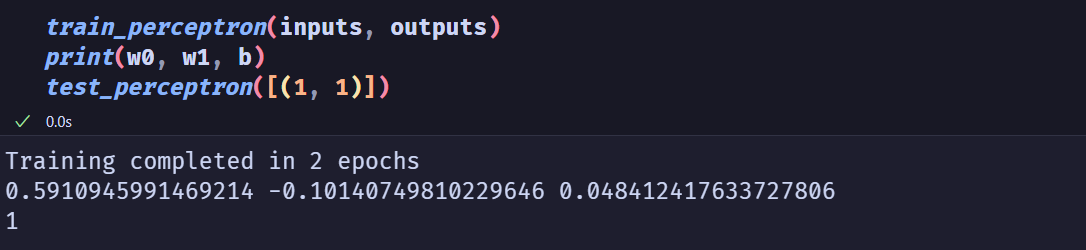
\includegraphics[width=\textwidth]{img/and.png}
    \caption{AND Gate Results}
    \label{fig:and_gate}
\end{figure}

\begin{figure}[ht]
    \centering
    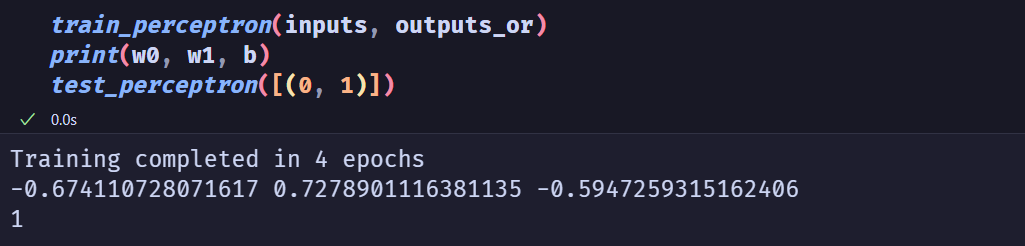
\includegraphics[width=\textwidth]{img/or.png}
    \caption{OR Gate Results}
    \label{fig:or_gate}
\end{figure}

\begin{figure}[ht]
    \centering
    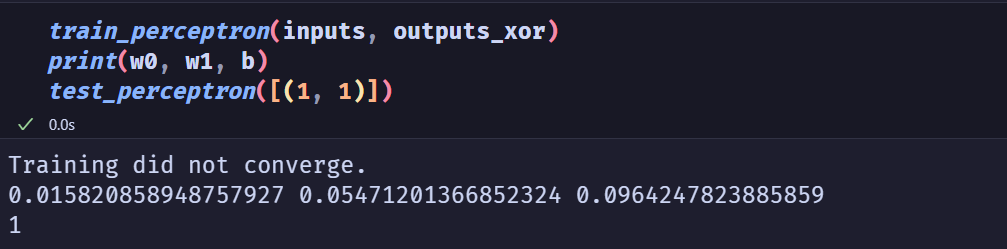
\includegraphics[width=\textwidth]{img/xor.png}
    \caption{XOR Gate Results}
    \label{fig:xor_gate}
\end{figure}

\section*{Discussion}

\subsection*{Why the XOR Problem Cannot Be Solved by a Single-Layer Perceptron}
The XOR (exclusive OR) gate is a classic example of a problem that cannot be solved by a single-layer perceptron. This is because the XOR function is not linearly separable; there is no straight line that can separate the output classes in the input space. A single-layer perceptron can only learn problems where such a linear boundary exists, like AND or OR gates. As a result, the perceptron fails to correctly classify all possible inputs for the XOR gate.

\subsection*{Role of the Logistic Function}
The logistic function, also known as the sigmoid function, is commonly used as an activation function in neural networks. It introduces non-linearity into the model, allowing the perceptron to learn more complex patterns than a simple linear model. However, even with a non-linear activation function like the logistic function, a single-layer perceptron still cannot solve the XOR problem due to its inherent linear structure. To overcome this limitation, multi-layer perceptrons (MLPs) are used, which stack multiple layers of perceptrons and can learn non-linear decision boundaries, making it possible to solve the XOR problem and other complex tasks.
\section*{Conclusion}
The Perceptron Learning Algorithm is a foundational concept in machine learning and neural networks. It provides a simple yet effective way to learn linear decision boundaries. However, its limitations in handling non-linearly separable data highlight the need for more advanced architectures, such as multi-layer perceptrons and deep learning models.
The implementation of the perceptron learning algorithm in Python demonstrates its practical application to basic logic gates. Future work could involve exploring more complex datasets and architectures to further enhance the capabilities of neural networks.



\end{document}